%----------------------------------------------------------------------------
We examine a three $\pi$ pulse sequence. Each pulse has the temporal profile (\ref{gaussian}) with $\sigma_\alpha=\sigma_\beta=\sigma_\gamma=2$ and $A=B=C=0.737832313319$. The centers of each pulse were placed symmetrically in the interval $[0,30]$: $t_\alpha=5$, $t_\beta=15$, and $t_\gamma=25$. For each run the amplitudes are selected in a uniform random fashion on the interval $[-20\%,+20\%]$ using the ``runif'' random number generator in MathCAD. Then a fourth-order Runge-Kutta fixed-step method is used to find the solution at 5001 points in the interval, and hence the residue ($\Psi_{residue}$) for each run. See figure \ref{three pi}.
%----------------------------------------------------------------------------
%----------------------------------------------------------------------------
% three_pi.tex
% by Troy Hix, April 2005
%----------------------------------------------------------------------------
\begin{figure}
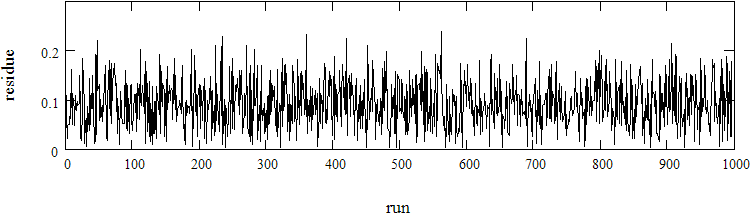
\includegraphics[width=6.00in]
{three_pi/three_pi.png}\\
\caption[Residue for runs using three $\pi$ pulses]{Residue for runs using three $\pi$ pulses. Three pulses of the form shown is figure \ref{solution one} were used at $t_\alpha=5$, $t_\beta=15$, and $t_\gamma=25$. The pulse amplitudes $A$, $B$, and $C$ varied uniformly on the interval $[-20\%,+20\%]$ for 1000 runs.}
\label{three pi}
\end{figure} 
%----------------------------------------------------------------------------
%

%----------------------------------------------------------------------------
%----------------------------------------------------------------------------
%----------------------------------------------------------------------------
%----------------------------------------------------------------------------
%----------------------------------------------------------------------------
%----------------------------------------------------------------------------
